\documentclass[12pt]{report}
\usepackage{amsmath}
\usepackage{graphicx}
\usepackage{listings}
\usepackage{caption}
\usepackage{hyperref}
\usepackage{xcolor} % Use xcolor instead of color
\usepackage{tikz}
\usepackage{graphicx}
\usepackage{float}


\lstdefinestyle{mypython}{
	language=Python,
	basicstyle=\ttfamily\footnotesize,
	keywordstyle=\color{blue},
	stringstyle=\color{red},
	commentstyle=\color{green},
	numbers=left,
	numberstyle=\tiny\color{gray},
	stepnumber=1,
	numbersep=10pt,
	backgroundcolor=\color{lightgray}, % lightgray is now defined
	frame=single,
	breaklines=true,
	showstringspaces=false
}

\begin{document}
	
	\title{Finite Element Analysis Report}
	\author{Hamidreza Owji}
	\maketitle
	
	\begin{abstract}
		This report presents the implementation and results of a finite element analysis (FEA) for various types of elements including Constant Strain Triangle (CST), Linear Strain Triangle (LST), Constant Strain Rectangle (CSR), Linear Strain Rectangle, and Constant Strain Hexahedra (CSH). The primary focus is on the CST elements, detailing the methodology, implementation, and results. Similar structures are followed for other elements.
	\end{abstract}
	
	\tableofcontents
	\listoffigures
	\listoftables
	
	\chapter{Introduction}
	Finite Element Analysis (FEA) is a powerful numerical technique used to solve complex structural, fluid, and thermal problems by discretizing the domain into smaller elements. This report focuses on the implementation of FEA for different types of elements, with a detailed examination of Constant Strain Triangle (CST) elements. The objective is to understand the behavior of materials under various conditions and compare the results for different element types.
	
	\chapter{Methodology}
	\section{Finite Element Method (FEM) Principles}
	The Finite Element Method (FEM) involves breaking down a complex domain into smaller, simpler parts called elements. Each element is defined by nodes, and the relationships between nodal displacements and element strains are captured by matrices such as the B matrix and the D matrix.
	
	\section{Types of Elements}
	This report considers the following types of elements:
	\begin{itemize}
		\item Constant Strain Triangle (CST)
		\item Linear Strain Triangle (LST)
		\item Constant Strain Rectangle (CSR)
		\item Linear Strain Rectangle (LSR)
		\item Constant Strain Hexahedra (CSH)
	\end{itemize}
	
	\section{Mathematical Formulations}
	\subsection{B Matrix}
	The B matrix bridges the gap between the physical displacements of the nodes and the strains in the material. It is derived from the shape functions of the element.
	
	\subsection{D Matrix}
	The D matrix, or material matrix, relates the stress and strain in the material, defined by the material properties such as Young's modulus and Poisson's ratio.
	
	\chapter{Constant Strain Triangle (CST) Elements}
	\section{Implementation}
	\subsection{Code Structure}
	The code for CST elements is structured into several modules, each responsible for different aspects of the FEA process. The primary modules are:
	\begin{itemize}
		\item FEM\_CST\_general
		\item Mesh\_Tri3\_extractor
		\item FEM\_CST\_plotting
	\end{itemize}
	
	\subsection{Key Functions}
	\subsubsection{Computing the B Matrix}
	\begin{lstlisting} [style=mypython][language=Python, caption={compute\_area\_and\_B\_matrix function}]
def compute_area_and_B_matrix(coords):
	"""Compute the area and B matrix for a CST element."""
	A = 0.5 * abs(coords[0][0]*(coords[1][1]-coords[2][1]) +
	coords[1][0]*(coords[2][1]-coords[0][1]) +
	coords[2][0]*(coords[0][1]-coords[1][1]))
	
	b = np.array([coords[1][1]-coords[2][1], coords[2][1]-coords[0][1], coords[0][1]-coords[1][1]])
	c = np.array([coords[2][0]-coords[1][0], coords[0][0]-coords[2][0], coords[1][0]-coords[0][0]])
	
	B = np.zeros((3, 6))
	B[0, ::2] = b
	B[1, 1::2] = c
	B[2, ::2] = c
	B[2, 1::2] = b
	B /= (2*A)
	
	return A, B
	\end{lstlisting}
	
	\subsubsection{Computing the D Matrix}
	\begin{lstlisting}[style=mypython][language=Python, caption={compute\_D\_matrix function}]
def compute_D_matrix(E, nu):
	"""Compute the D matrix (material matrix)."""
	return E / (1-nu**2) * np.array([[1, nu, 0], [nu, 1, 0], [0, 0, (1-nu)/2]])
	\end{lstlisting}
	
	\subsubsection{Computing the Stiffness Matrix}
	\begin{lstlisting}[style=mypython][language=Python, caption={compute\_stiffness\_matrix function}]
def compute_stiffness_matrix(coords, D):
	"""Compute the stiffness matrix for a CST element."""
	A, B = compute_area_and_B_matrix(coords)
	return A * np.dot(B.T, np.dot(D, B))
	\end{lstlisting}
	
	\subsubsection{Assembling the Global Stiffness Matrix}
	\begin{lstlisting}[style=mypython][language=Python, caption={assemble\_global\_stiffness function}]
def assemble_global_stiffness(elements, D):
	"""Assemble the global stiffness matrix."""
	num_nodes = max([node for elem in elements for node in elem['nodes']])
	K_global = np.zeros((2*num_nodes, 2*num_nodes))
	
	for elem in elements:
	k = compute_stiffness_matrix(elem['coords'], D)
	for i in range(3):
	for j in range(3):
	m, n = elem['nodes'][i], elem['nodes'][j]
	K_global[2*m-2:2*m, 2*n-2:2*n] += k[2*i:2*i+2, 2*j:2*j+2]
	
	return K_global
	\end{lstlisting}
	
	\subsubsection{Computing Global Forces}
	\begin{lstlisting}[style=mypython][language=Python, caption={compute\_global\_forces function}]
def compute_global_forces(K_global, U):
	"""Compute the global forces from the global stiffness matrix and nodal displacements."""
	return np.dot(K_global, U)
	\end{lstlisting}
	
	\section{Full modules}
	\subsection{Mesh\_Tri3\_extractor.py}
	This module is responsible getting mesh information from MED file
	\begin{lstlisting}[style=mypython]
import h5py
import numpy as np

def divide_list_into_sublists(lst, n):
	for i in range(0, len(lst), n):
		yield lst[i:i + n]

def extract_coordinates(lst, number_of_coordinates):
	for i in range(0, len(lst), number_of_coordinates):
		yield lst[i:i + number_of_coordinates]
def generate_elements(node_coordinates, element_node_connectivity):
	elements = []
	for element in element_node_connectivity:
		element_dict = {
			'nodes': element,
			'coords': np.array([node_coordinates[node - 1] for node in element])
		}
		elements.append(element_dict)
	return elements
	
def read_mesh_data(file_name):
	with h5py.File(file_name, 'r') as file:
		# Read coordinate data
		coo_dataset = file['ENS_MAA/Mesh_1/-0000000000000000001-0000000000000000001/NOE/COO']
		coo_data = coo_dataset[:]
		num_nodes = len(coo_data) // 2
		subcoord = list(extract_coordinates(coo_data, num_nodes))
		node_coordinates = [group for group in zip(*subcoord)]
		
		# Read TRIA3/NOD dataset for TRIA3 elements
		tr3_dataset = file['ENS_MAA/Mesh_1/-0000000000000000001-0000000000000000001/MAI/TR3/NOD']
		tr3_data = tr3_dataset[:]
		num_triangles = len(tr3_data) // 3
		sublists = list(divide_list_into_sublists(tr3_data, num_triangles))
		element_node_connectivity = [group for group in zip(*sublists)]

	return node_coordinates, element_node_connectivity
	\end{lstlisting}
	
	\subsection{FEM\_CST\_general.py}
This module is responsible getting mesh information from MED file
\begin{lstlisting}[style=mypython]
import numpy as np
from Mesh_Tri3_extractor import generate_elements, read_mesh_data
from FEM_CST_plotting import (plot_mesh, plot_displacements, plot_mesh_with_boundary_conditions, plot_loads, plot_mesh_with_loads)

def compute_area_and_B_matrix(coords):
	"""Compute the area and B matrix for a CST element."""
	A = 0.5 * abs(coords[0][0]*(coords[1][1]-coords[2][1]) +
	coords[1][0]*(coords[2][1]-coords[0][1]) +
	coords[2][0]*(coords[0][1]-coords[1][1]))
	
	b = np.array([coords[1][1]-coords[2][1], coords[2][1]-coords[0][1], coords[0][1]-coords[1][1]])
	c = np.array([coords[2][0]-coords[1][0], coords[0][0]-coords[2][0], coords[1][0]-coords[0][0]])
	
	B = np.zeros((3, 6))
	B[0, ::2] = b
	B[1, 1::2] = c
	B[2, ::2] = c
	B[2, 1::2] = b
	B /= (2*A)
	
	return A, B

def compute_D_matrix(E, nu):
	"""Compute the D matrix (material matrix)."""
	return E / (1-nu**2) * np.array([[1, nu, 0], [nu, 1, 0], [0, 0, (1-nu)/2]])

def compute_stiffness_matrix(coords, D):
	"""Compute the stiffness matrix for a CST element."""
	A, B = compute_area_and_B_matrix(coords)
	return A * np.dot(B.T, np.dot(D, B))

def assemble_global_stiffness(elements, D):
	"""Assemble the global stiffness matrix."""
	num_nodes = max([node for elem in elements for node in elem['nodes']])
	K_global = np.zeros((2*num_nodes, 2*num_nodes))

	for elem in elements:
	k = compute_stiffness_matrix(elem['coords'], D)
	for i in range(3):
	for j in range(3):
	m, n = elem['nodes'][i], elem['nodes'][j]
	K_global[2*m-2:2*m, 2*n-2:2*n] += k[2*i:2*i+2, 2*j:2*j+2]
	
	return K_global
	
def compute_global_forces(K_global, U):
	"""Compute the global forces from the global stiffness matrix and nodal displacements."""
	return np.dot(K_global, U)

def compute_element_forces(element, U, D):
	"""Compute the element forces from the element stiffness matrix and nodal displacements."""
	k = compute_stiffness_matrix(element['coords'], D)
	u_element = np.array([U[2*node-2:2*node] for node in element['nodes']]).flatten()
	return np.dot(k, u_element)

def compute_element_stress(element, U, D):
	"""Compute the stress within an element."""
	u_element = np.array([U[2*node-2:2*node] for node in element['nodes']]).flatten()
	A, B = compute_area_and_B_matrix(element['coords'])
	epsilon = np.dot(B, u_element)
	sigma = np.dot(D, epsilon)
	return sigma

def compute_principal_stresses_and_angles(sigma):
	"""Compute the principal stresses from the stress vector."""
	sigma_x, sigma_y, tau_xy = sigma
	sigma_avg = 0.5 * (sigma_x + sigma_y)
	R = np.sqrt(((sigma_x - sigma_y) * 0.5)**2 + tau_xy**2)
	sigma_1 = sigma_avg + R
	sigma_2 = sigma_avg - R
	theta_rad = 0.5 * np.arctan2(2 * tau_xy, sigma_x - sigma_y)
	theta_deg = np.degrees(theta_rad)
	return sigma_1, sigma_2, theta_deg

# Example usage
E = 2.1e6  # Modulus of elasticity in Pa (for steel)
nu = 0.3  # Poisson's ratio (for steel)
D = compute_D_matrix(E, nu)  # Compute D matrix once and reuse

node_coordinates, element_node_connectivity = read_mesh_data('Mesh_1.med')
elements = generate_elements(node_coordinates, element_node_connectivity)

K_global = assemble_global_stiffness(elements, D)
# print(K_global)

# Identify boundary nodes and apply conditions. This gives us index not node number
left_boundary_nodes = [node + 1 for node, coord in enumerate(node_coordinates) if coord[0] == 0]
# print('left boundary: ', left_boundary_nodes)

# Initialize the displacement vector with zeros (as a starting assumption)
U = np.zeros(2 * len(node_coordinates))

# Identify nodes with x=140 and apply a load of 1000 in the x direction
F_external = np.zeros_like(U)

# Node index where the load will be applied (Python uses 0-based indexing, so node 3 is indexed as 2)
node_index = 3 - 1 # Adjust for 0-based indexing by subtracting 1

# Apply a load of 1000 in the x direction to node 3
F_external[2*node_index + 1] = -1000  # Apply load in x direction. For y direction, use 2*node_index + 1

# print('f external: ', F_external)

fixed_dof = []
for node in left_boundary_nodes:  # assuming left_boundary_nodes contain fixed nodes
	fixed_dof.extend([2*(node -1), 2*(node -1) +1])

K_reduced = np.delete(K_global, fixed_dof, axis=0)  # Remove rows
K_reduced = np.delete(K_reduced, fixed_dof, axis=1)  # Remove columns
F_reduced = np.delete(F_external, fixed_dof)
# print('f reduced: ', F_reduced)
U_reduced = np.linalg.solve(K_reduced, F_reduced)
U_full = np.zeros_like(U)
free_dof = set(range(len(U))) - set(fixed_dof)
free_dof = list(free_dof)
U_full[free_dof] = U_reduced


F_global_calculated = compute_global_forces(K_global, U_full)

# Uncomment the following lines for debugging:
# print("Global Forces:")
# print(F_global_calculated)

# Uncomment the following blocks for debugging:
# for elem in elements:
#     F_element = compute_element_forces(elem, U_full, D)  
#     print(f"Element Forces for nodes {elem['nodes']}:")
#     print(F_element)

# for elem in elements:
#     sigma_element = compute_element_stress(elem, U_full, D)  
#     print(f"Element Stress for nodes {elem['nodes']}:")
#     print(sigma_element)

# for elem in elements:
#     sigma_element = compute_element_stress(elem, U_full, D) 
#     sigma_1, sigma_2, theta_deg = compute_principal_stresses_and_angles(sigma_element)
#     print(f"Principal Stresses for element with nodes {elem['nodes']}:")
#     print(f"Maximum (sigma_1): {sigma_1}")
#     print(f"Minimum (sigma_2): {sigma_2}")
#     print(f"Angle of Maximum Stress (degrees): {theta_deg}")

# for i, coord in enumerate(node_coordinates):
#     x, y = coord  # Unpack the x and y coordinates of the node
#     dx = U_full[2*i]   # x displacement of node i
#     dy = U_full[2*i+1] # y displacement of node i
#     print(f"Node {i+1}: x = {x:.6f}, y = {y:.6f}, dx = {dx:.6f}, dy = {dy:.6f}")

# print('max dis= ', max(U_full))
plot_displacements(node_coordinates, U_full, 'Nodal Displacements', scale_factor=1000)
# print(U_full)
# plot_mesh(elements, node_coordinates)
# plot_displacements(node_coordinates, U, 'stress')

# plot_mesh_with_boundary_conditions(elements, node_coordinates, left_boundary_nodes)
# plot_loads(node_coordinates, F_external, 1)
# plot_mesh_with_loads(elements, node_coordinates, left_boundary_nodes, F_external)

# Assuming U_full is already defined and contains the displacements for each node
displacement_magnitudes = np.sqrt(U_full[::2]**2 + U_full[1::2]**2)

max_disp_node_index = np.argmax(displacement_magnitudes)

max_disp_magnitude = displacement_magnitudes[max_disp_node_index]

max_disp_node_number = max_disp_node_index + 1

max_disp_x = U_full[2*max_disp_node_index]
max_disp_y = U_full[2*max_disp_node_index + 1]

# Print the information
print(f"Node with Maximum Displacement: Node {max_disp_node_number}")
print(f"Displacement in X: {max_disp_x:.6f}")
print(f"Displacement in Y: {max_disp_y:.6f}")
print(f"Total Displacement Magnitude: {max_disp_magnitude:.6f}")

\end{lstlisting}
\begin{figure}[h]
	\centering
	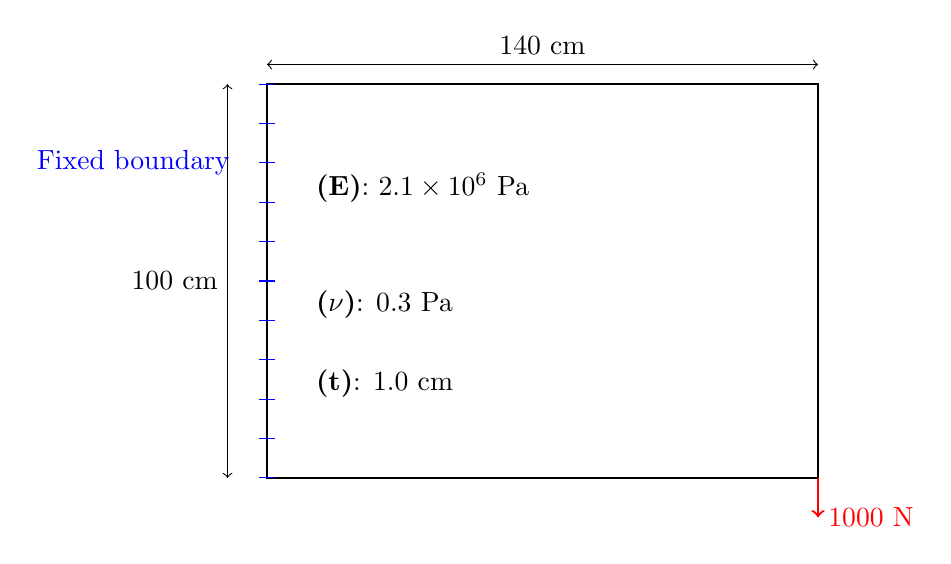
\begin{tikzpicture}[scale=0.5] % Adjust the scale to fit the page
		% Draw the rectangle
		\draw[thick] (0,0) rectangle (14,10);
		
		% Label dimensions
		\draw[<->] (0,10.5) -- (14,10.5) node[midway,above] {140 cm};
		\draw[<->] (-1,0) -- (-1,10) node[midway,left] {100 cm};
		
		% Draw load arrow
		\draw[->, red, thick] (14,0) -- (14,-1) node[anchor=west] {1000 N}; % Corrected arrow direction
		
		% Boundary condition
		\foreach \y in {0,1,...,10} {
			\draw[blue] (-0.2,\y) -- (0.2,\y);
		}
		\node[anchor=east, blue] at (-0.7, 8) {Fixed boundary}; % Adjusted position
		
		\node[anchor=north west] at (1,8) {
			\textbf{(E)}: \(2.1 \times 10^6\) Pa
		};

		\node[anchor=north west] at (1,5) {
			\textbf{(\(\nu\))}: 0.3 Pa
		};

		\node[anchor=north west] at (1,3) {
			\textbf{(t)}: 1.0 cm
		};
	\end{tikzpicture}
	\caption{Finite Element Analysis of a Rectangular Steel Plate}
	\label{fig:fea-plate}
\end{figure}


\subsection{Problem Description}
In this example, we analyze a rectangular steel plate with dimensions 100 cm by 140 cm. The plate has the following properties and loading conditions:
\begin{itemize}
	\item \textbf{Modulus of Elasticity (E)}: \(2.1 \times 10^6\) Pa (typical for steel)
	\item \textbf{Poisson's Ratio (\(\nu\))}: 0.3 (typical for steel)
	\item \textbf{External Load}: A load of 1000 N applied in the x-direction at a node located at \(x = 140\) cm and \(y = 0\) cm.
\end{itemize}

The material matrix \(D\) is computed using the given modulus of elasticity and Poisson's ratio. The mesh data, including node coordinates and element connectivity, is read from a file named \texttt{Mesh\_1.med}. Using this mesh data, elements are generated and the global stiffness matrix is assembled.

Boundary conditions are applied to nodes located at \(x = 0\) cm (left boundary), and the external load is applied to the specified node.

\subsection{Mesh and Boundary Conditions}
The following Python code demonstrates the steps for setting up and solving the FEA problem:

\begin{figure}[H]
	\centering
	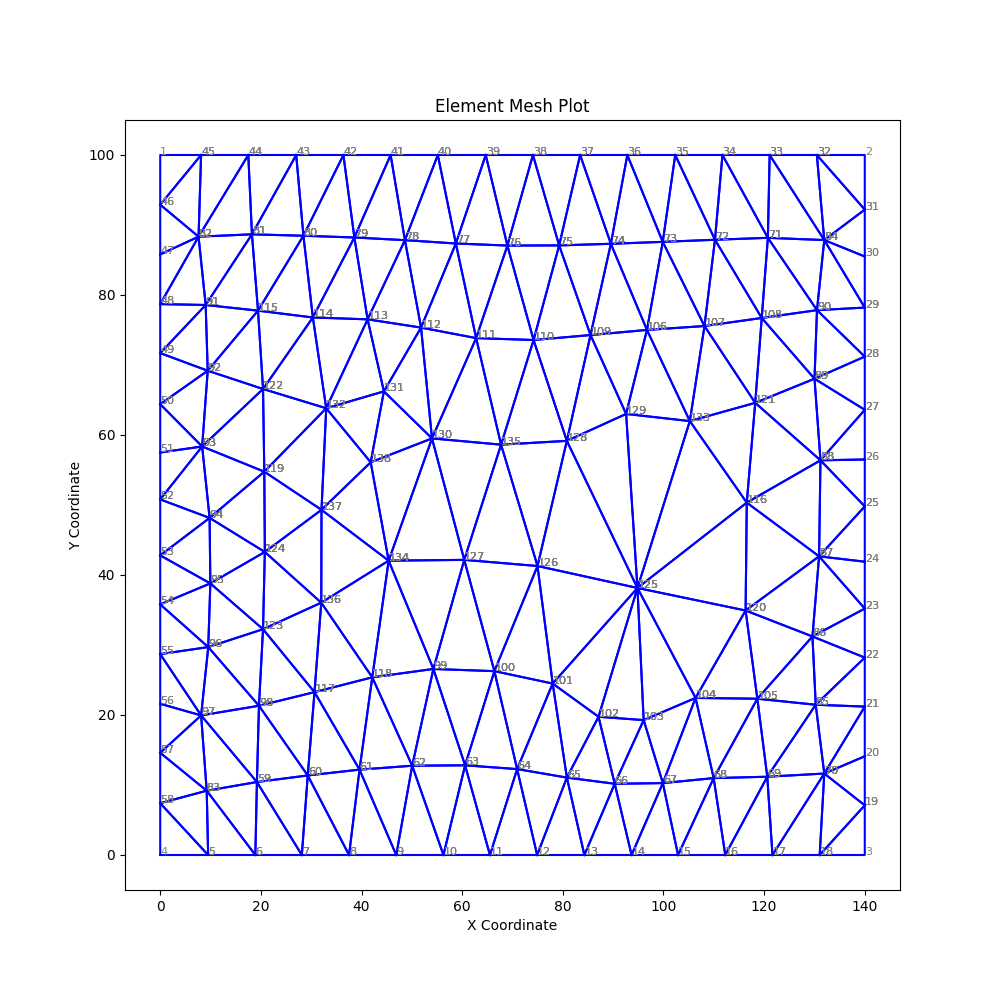
\includegraphics[width=0.8\textwidth]{mesh.png} % Adjust the width as needed
	\caption{Generated mesh by Salome}
	\label{fig:generated mesh}
\end{figure}

\begin{lstlisting}[style=mypython, caption={Python code for setting up the FEA problem}]
	E = 2.1e6  # Modulus of elasticity in Pa (for steel)
	nu = 0.3  # Poisson's ratio (for steel)
	D = compute_D_matrix(E, nu)  # Compute D matrix once and reuse
	
	node_coordinates, element_node_connectivity = read_mesh_data('Mesh_1.med')
	elements = generate_elements(node_coordinates, element_node_connectivity)
	
	K_global = assemble_global_stiffness(elements, D)
	
	# Identify boundary nodes and apply conditions. This gives us index not node number
	left_boundary_nodes = [node + 1 for node, coord in enumerate(node_coordinates) if coord[0] == 0]
	
	# Initialize the displacement vector with zeros (as a starting assumption)
	U = np.zeros(2 * len(node_coordinates))
	
	# Identify nodes with x=140 and apply a load of 1000 in the x direction
	F_external = np.zeros_like(U)
	
	# Node index where the load will be applied (Python uses 0-based indexing, so node 3 is indexed as 2)
	node_index = 3 - 1 # Adjust for 0-based indexing by subtracting 1
	
	# Apply a load of 1000 in the x direction to node 3
	F_external[2*node_index + 1] = -1000  # Apply load in x direction. For y direction, use 2*node_index + 1
\end{lstlisting}
	

\begin{figure}[H]
	\centering
	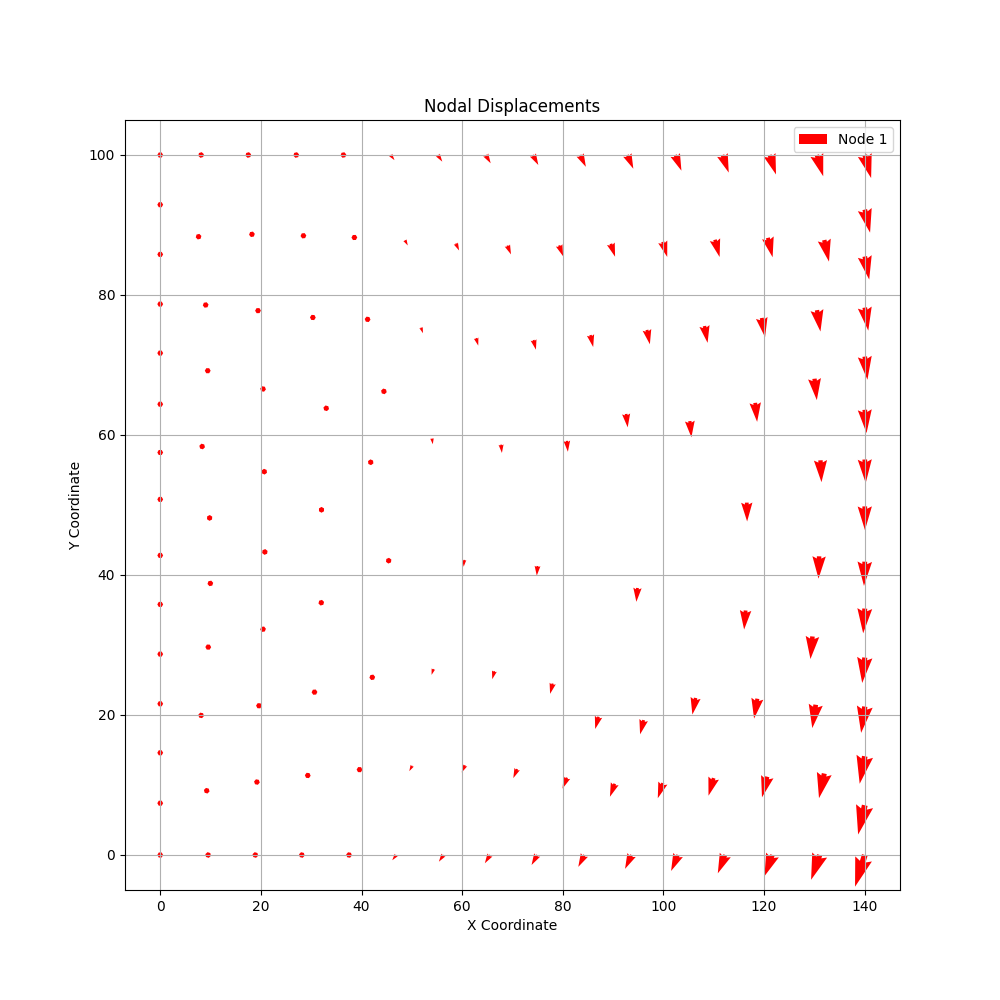
\includegraphics[width=0.8\textwidth]{displacement.png} % Adjust the width as needed
	\caption{Generated mesh by Salome}
	\label{fig:generated mesh}
\end{figure}

\subsection{Results}
\begin{tabular}{|l|l|}
	\hline
	\textbf{Node with Maximum Displacement} & Node 3 \\ \hline
	\textbf{Displacement in X} & -0.003867 \\ \hline
	\textbf{Displacement in Y} & -0.009054 \\ \hline
	\textbf{Total Displacement Magnitude} & 0.009845 \\ \hline
\end{tabular}
	
	\section{Discussion}
	% Analyze and discuss the results here
	The results for CST elements show that...
	
	\chapter{Linear Strain Triangle (LST) Elements}
	\section{Implementation}
	% Similar structure as for CST elements
	
	\section{Results}
	% Include plots and results here
	
	\section{Discussion}
	% Analyze and discuss the results here
	
	\chapter{Constant Strain Rectangle (CSR) Elements}
	\section{Implementation}
	% Similar structure as for CST elements
	
	\section{Results}
	% Include plots and results here
	
	\section{Discussion}
	% Analyze and discuss the results here
	
	\chapter{Linear Strain Rectangle (LSR) Elements}
	\section{Implementation}
	% Similar structure as for CST elements
	
	\section{Results}
	% Include plots and results here
	
	\section{Discussion}
	% Analyze and discuss the results here
	
	\chapter{Constant Strain Hexahedra (CSH) Elements}
	\section{Implementation}
	% Similar structure as for CST elements
	
	\section{Results}
	% Include plots and results here
	
	\section{Discussion}
	% Analyze and discuss the results here
	
	\chapter{Conclusion}
	% Summarize the findings and suggest future work
	
	\chapter{References}
	% List of references
	
	\appendix
	\chapter{Code}
	\section{Full Code}
	% Include full code or additional snippets here
	
\end{document}
